%%    _____  _____
%%   |  __ \|  __ \    AUTHOR: Pedro Rivero
%%   | |__) | |__) |   ---------------------------------
%%   |  ___/|  _  /    DATE: November 10, 2021
%%   | |    | | \ \    ---------------------------------
%%   |_|    |_|  \_\   https://github.com/pedrorrivero
%%

\section{Solving NJL}

%% ----------------------------------------------------------------------------
%% ----------------------------------------------------------------------------

\begin{frame}[allowframebreaks]{Quantum computing the NJL model}

  \begin{itemize}
    \item<1-> Since we would like to study both the ground state, as well as the first excited hadron state in NJL, we will be using SSVQE as our variational algorithm.
    \item<2-> Using HVA we can use the fact that adiabatic state preparation maps corresponding excited states, to raise our chances of getting the correct output eigenstates in SSVQE without need for redundancy.
    \item<3-> HVA's parametrization is based on the system's Hamiltonian, it will share its symmetries. This means that we can easily use SSVQE to get non-consecutive output eigenstates by simply using non-consecutive initial eigenstates.
    \item<4-> HVA requires breaking up our Hamiltonian into its non-commuting components.
  \end{itemize}


%% ----------------------------------------------------------------------------
\break
%% ----------------------------------------------------------------------------

  \begin{align*}
    H_{N}^{(1)} \quad\defeq\quad&
      \frac{1}{4a} \sum_\alpha \sum_{n=\text{even}}^{2N-1}
      \qty[
        \sigma_\alpha^{1}(n+1) \sigma_\alpha^{2}(n) -
        \sigma_\alpha^{2}(n+1) \sigma_\alpha^{1}(n)
      ] \qc\\
    H_{N}^{(2)} \quad\defeq\quad& - \frac{G_{\pi}}{2a} \sum_{n=0}^{N-1} \qty[
      \sum_{\alpha} \dbtilde{H}_{N}^{\alpha\alpha}(n) + 2
      \sum_{\alpha < \beta} \dbtilde{H}_{N}^{\alpha\beta}(n)] \qc\\
    H_{N}^{(3)} \quad\defeq\quad&
      \frac{1}{4a} \sum_\alpha \sum_{n=\text{odd}}^{2N-2}
      \qty[
        \sigma_\alpha^{1}(n+1) \sigma_\alpha^{2}(n) -
        \sigma_\alpha^{2}(n+1) \sigma_\alpha^{1}(n)
      ] + \nonumber\\&
      \frac{1}{4a} \sum_\alpha \!
      \qty[\prod_{l=1}^{2N-2} \!\! \sigma_\alpha^3(l)] \!
      \qty[
        \sigma_\alpha^{1}(0) \sigma_\alpha^{2}(2N \!-\! 1) -
        \sigma_\alpha^{2}(0) \sigma_\alpha^{1}(2N \!-\! 1)
      ] \qc\\
    H_{N}^{(4)} \quad\defeq\quad&
      \frac{m}{2} \sum_\alpha \sum_{n=0}^{2N-1}
      (-1)^{n+1}\sigma_\alpha^{3}(n) \qc
  \end{align*}

%% ----------------------------------------------------------------------------
\break
%% ----------------------------------------------------------------------------

  \begin{minipage}[c]{\linewidth}\begin{multicols}{2}

    We choose the mass term for the initial states:

    \begin{gather*}
      H_{N}^{(4)} \;\defeq\;
        \frac{m}{2} \sum_\alpha \sum_{n=0}^{2N-1}
        (-1)^{n+1}\sigma_\alpha^{3}(n)
    \end{gather*}

    \begin{itemize}
      \item<1-> Ground: $\ket{\Omega_0} \defeq \ket{\bin...1010101010}$
      \item<1-> Hadron: $\ket{h_0} \defeq \ket{\bin...1010101001} + \cdots$
    \end{itemize}

    Where we can build the initial hadron state by implementing \textbf{Dicke states}:

    \begin{center}
      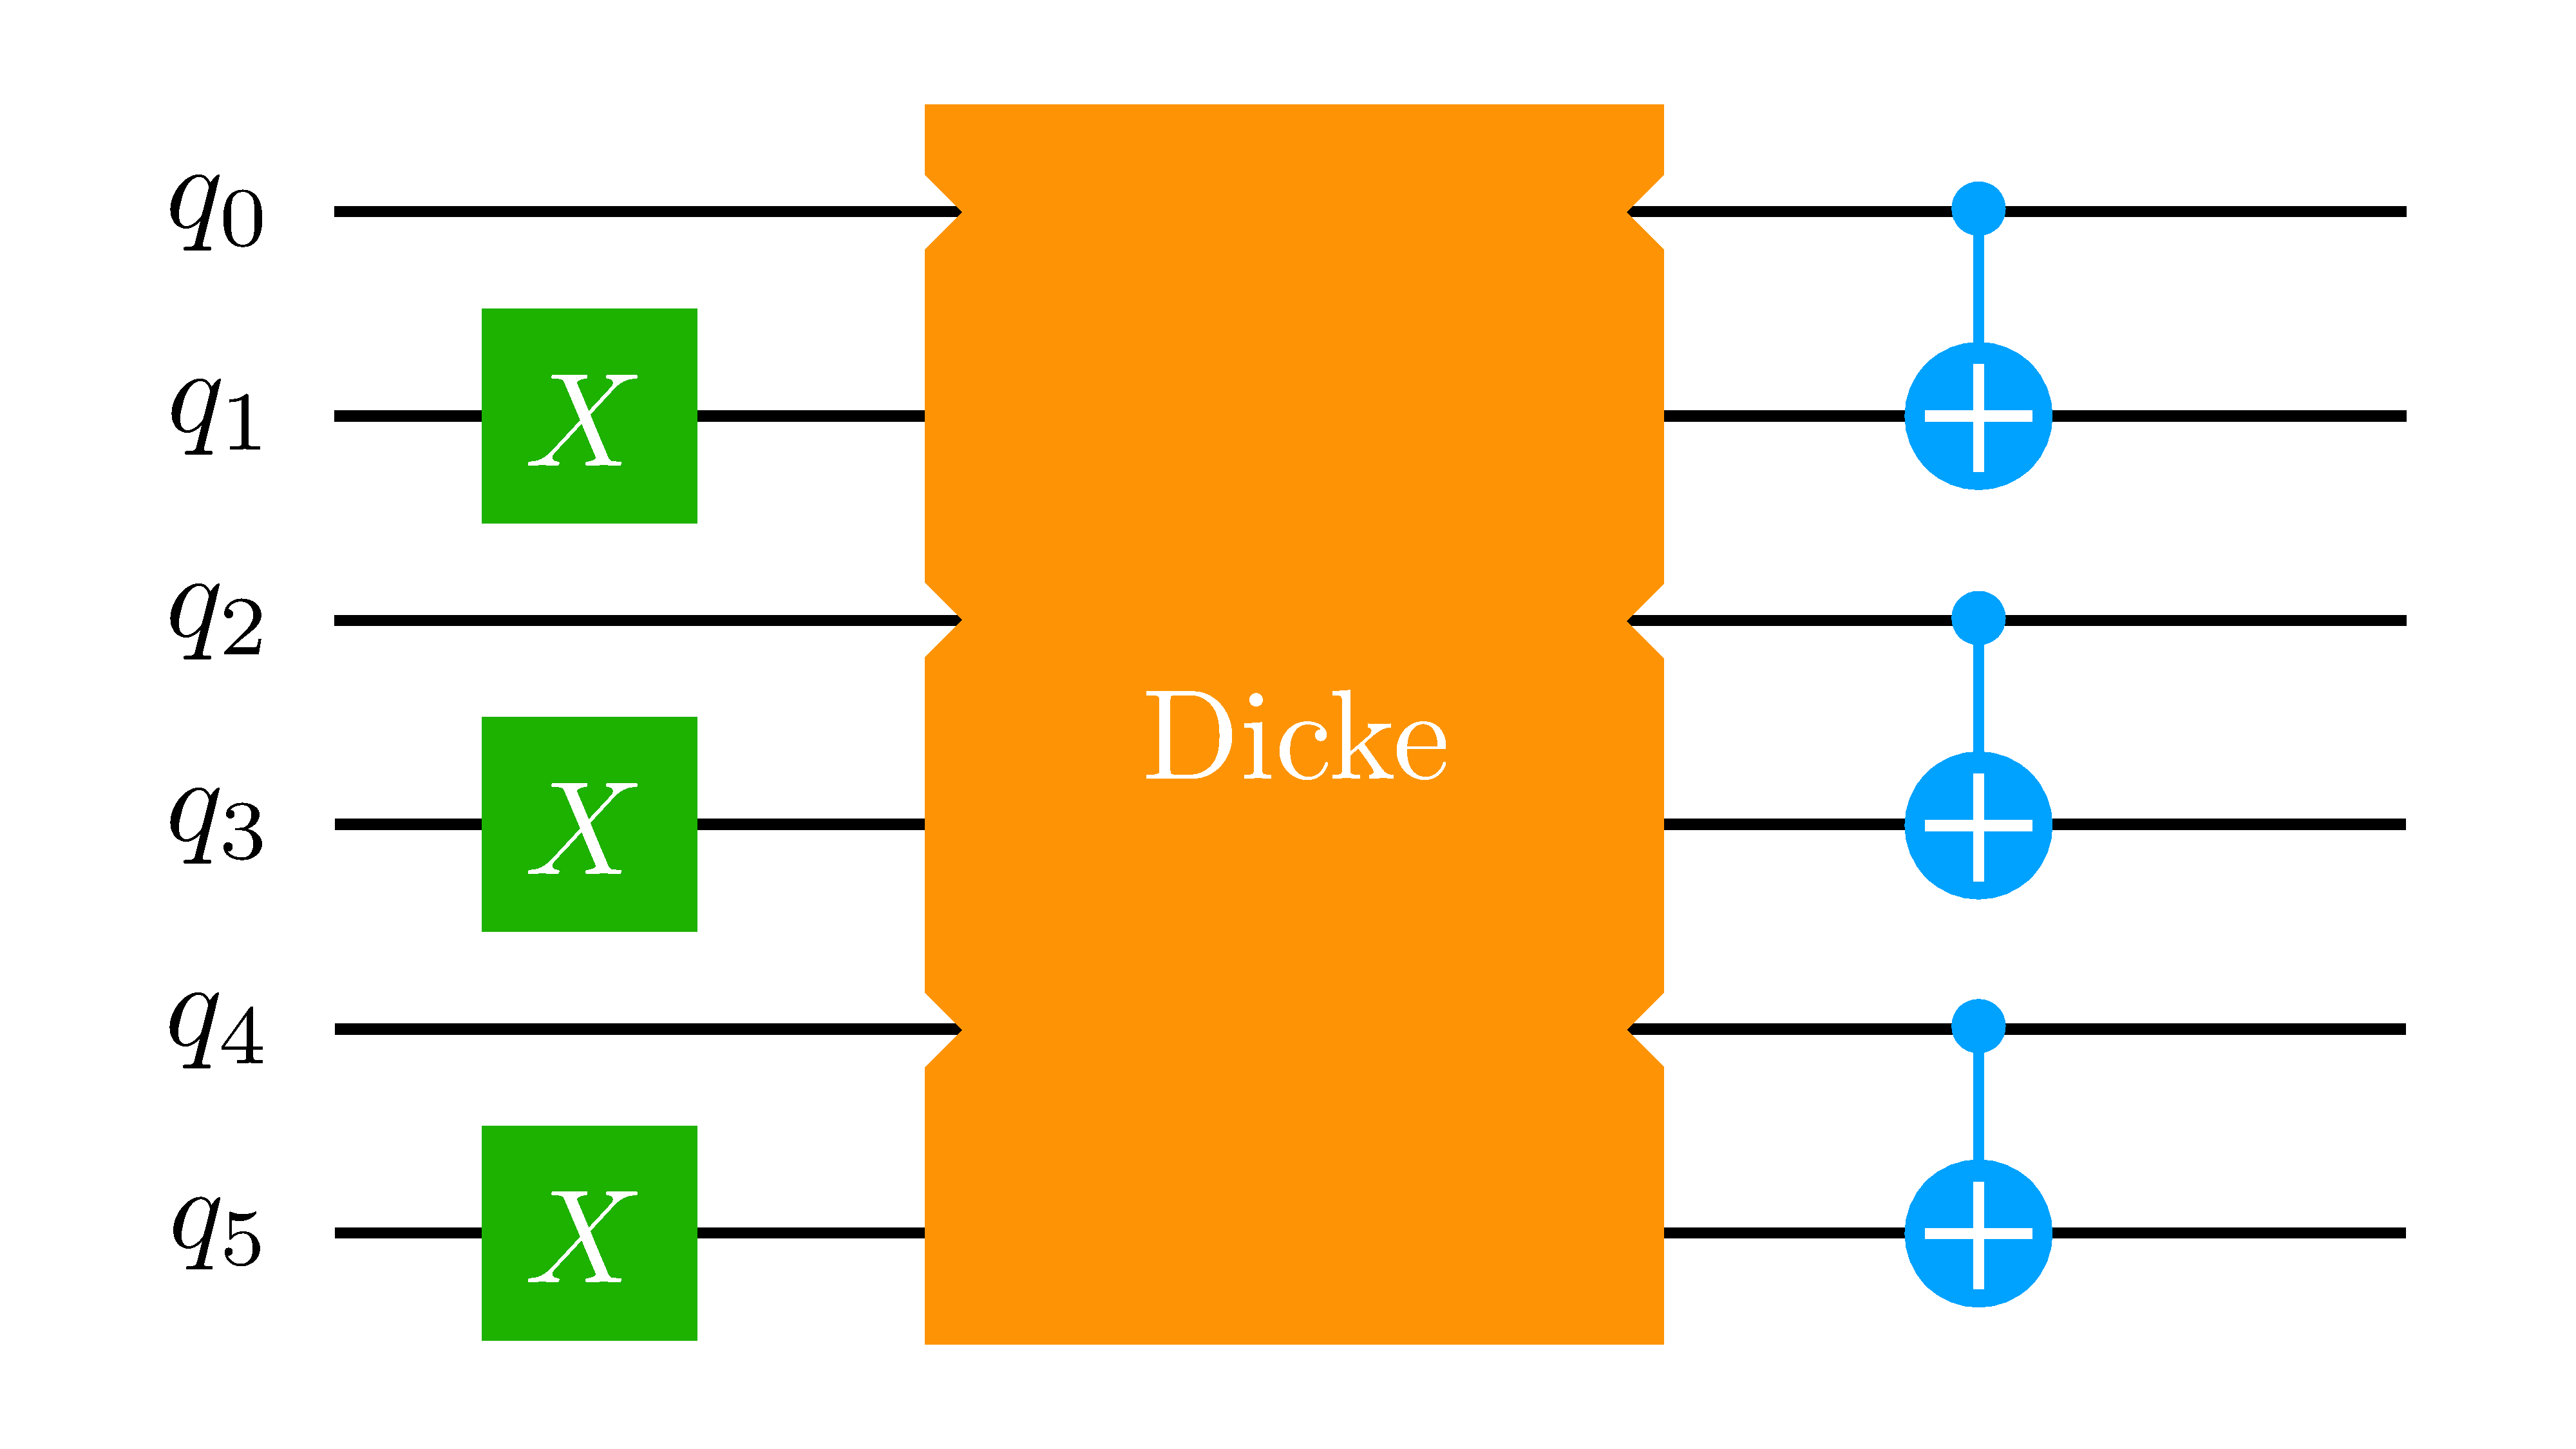
\includegraphics[width=.25\paperwidth]{Figures/chapter06/hadron-init}
    \end{center}

    \vfill
    \columnbreak

    \begin{center}
      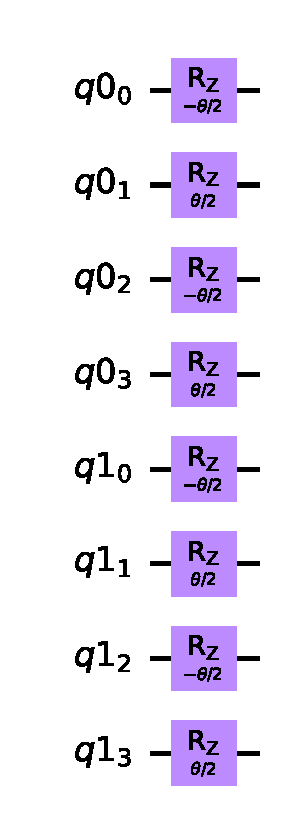
\includegraphics[width=.15\paperwidth]{Figures/chapter06/H4-rotation}
    \end{center}

  \end{multicols}\end{minipage}

%% ----------------------------------------------------------------------------
\break\break
%% ----------------------------------------------------------------------------

  \begin{minipage}[c]{\linewidth}
  \begin{gather*}
    H_{N}^{(2)} \;\defeq\; - \frac{G_{\pi}}{2a} \sum_{n=0}^{N-1} \qty[
      \sum_{\alpha} \dbtilde{H}_{N}^{\alpha\alpha}(n) + 2
      \sum_{\alpha < \beta} \dbtilde{H}_{N}^{\alpha\beta}(n)] \\
    \dbtilde{H}_{N}^{\alpha\beta}(n) \qra
    \frac{1}{4} \sum_{{j=0}\atop{k=0}}^{1}
    (-1)^{j+k} \, \sigma_\alpha^{3}(2n+j) \, \sigma_\beta^{3}(2n+k) \
  \end{gather*}
  \vspace{-2em}
  \begin{center}
    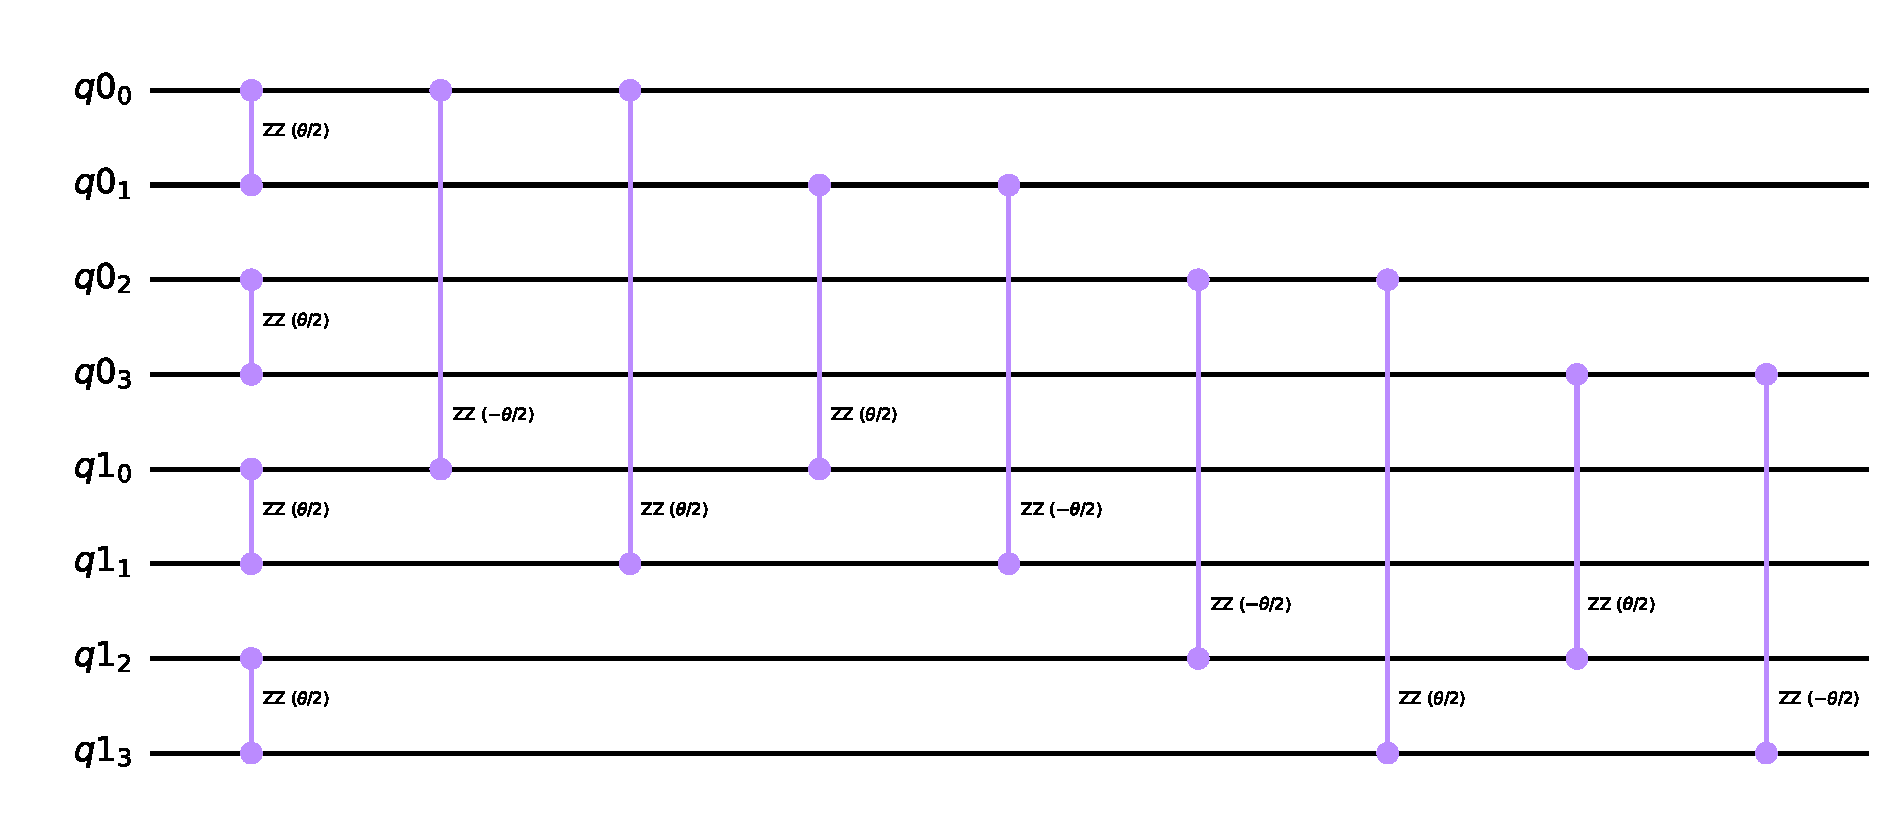
\includegraphics[width=.60\paperwidth]{Figures/chapter06/H2-rotation}
  \end{center}
  \vspace{-2em}
\end{minipage}


%% ----------------------------------------------------------------------------
\break
%% ----------------------------------------------------------------------------

  The kinetic terms of the form $XY-YX$ can be easily exponentiated by noting that:

  \begin{multicols}{2}

    \begin{gather*}
      \frac{1}{2}(X_1Y_0 - Y_1X_0) =
      \mqty[\phpl 0 & \phpl 0 & \phpl 0 & \phpl 0 \\
            \phpl 0 & \phpl 0 & \phpl i & \phpl 0 \\
            \phpl 0 &      -i & \phpl 0 & \phpl 0 \\
            \phpl 0 & \phpl 0 & \phpl 0 & \phpl 0   ] \qc
    \end{gather*}

    \begin{itemize}
      \item Zero eigenvalue on even parity states: single particle/antiparticle states
      \item Pauli~Y in the subspace $\qty{\ket{\bin 10}, \ket{\bin 01}}$: creates and annihilates particle-antiparticle pairs.
    \end{itemize}

  \columnbreak

    \begin{center}
      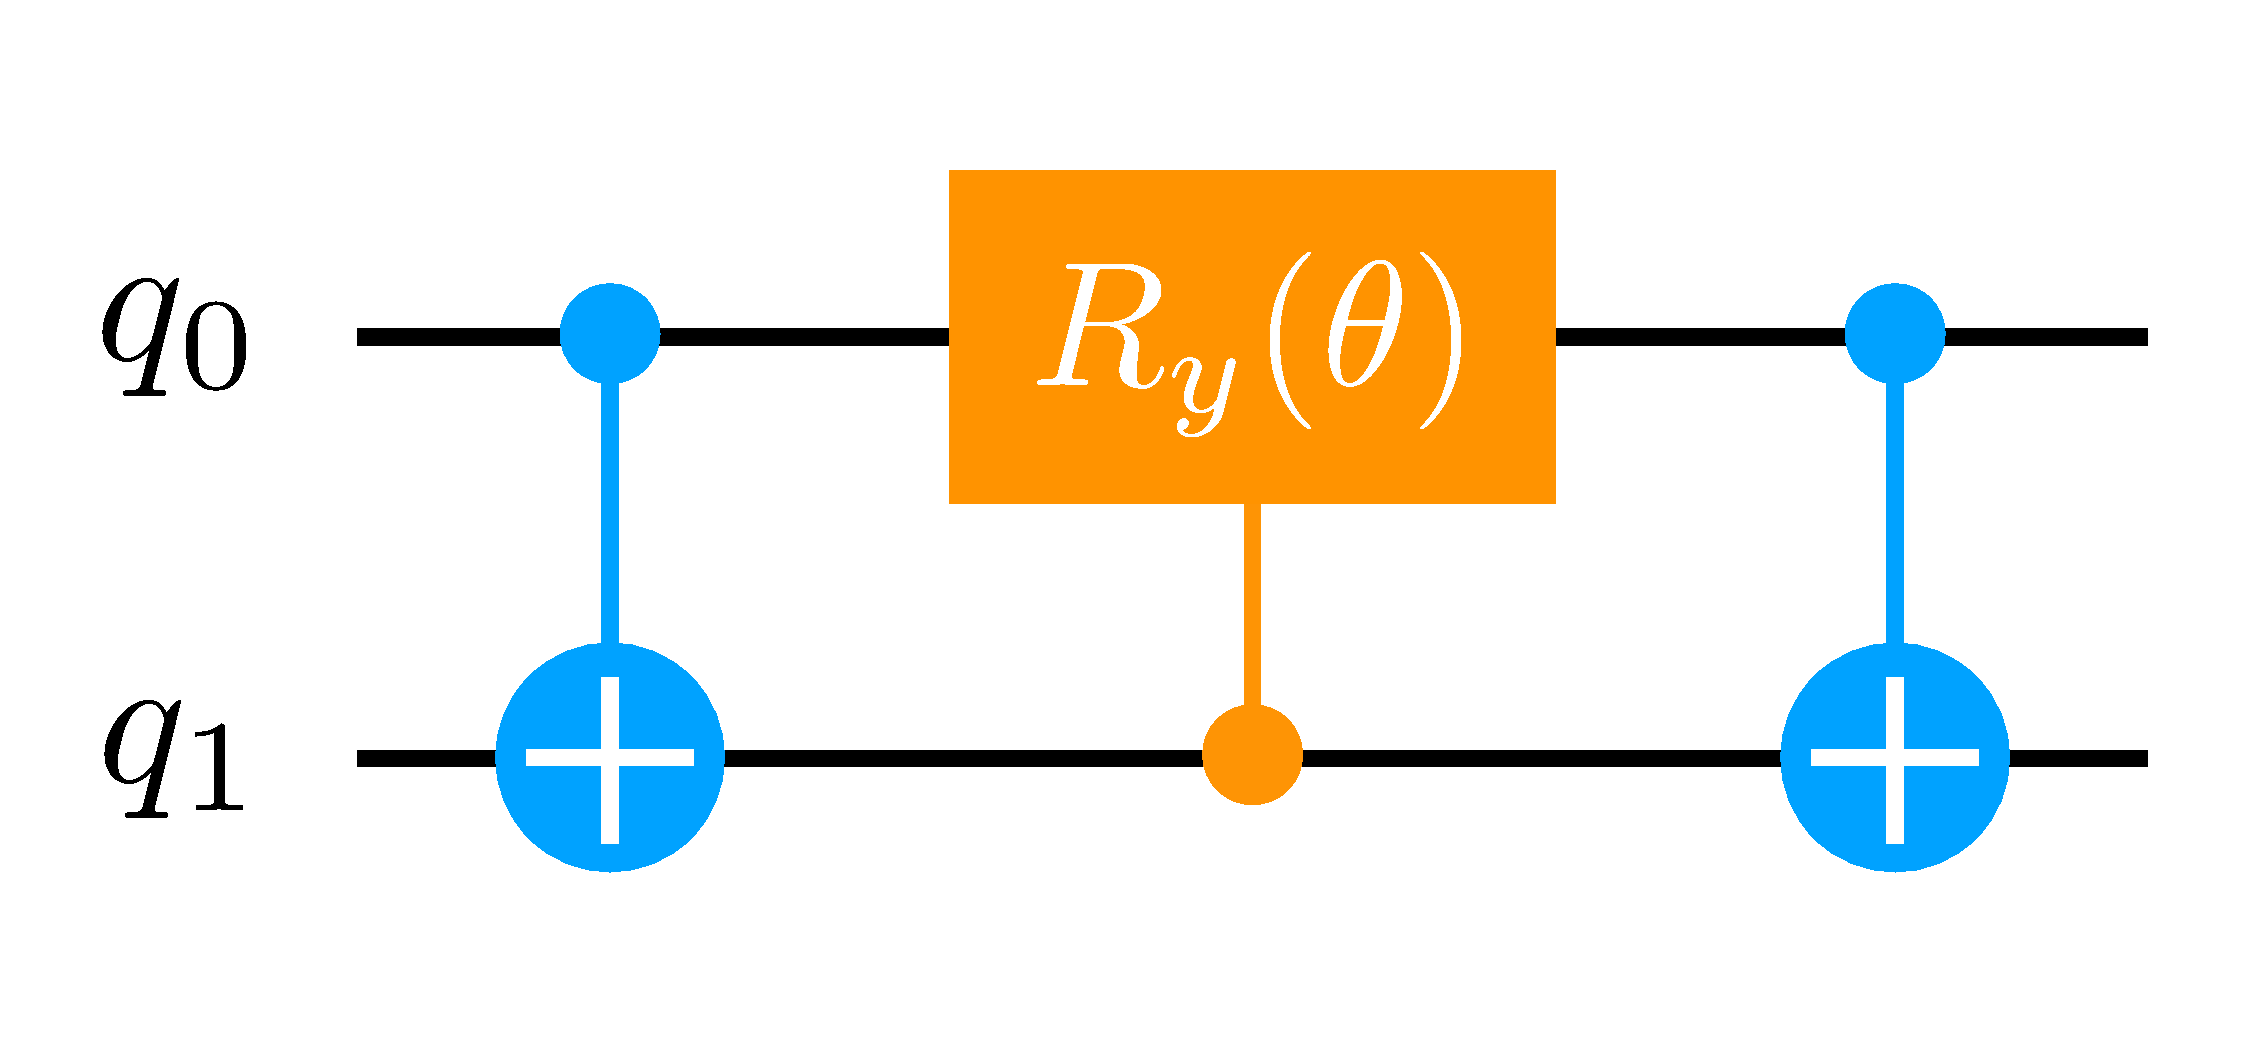
\includegraphics[width=.25\paperwidth]{Figures/chapter06/xy-rotation}
    \end{center}

    \begin{center}
      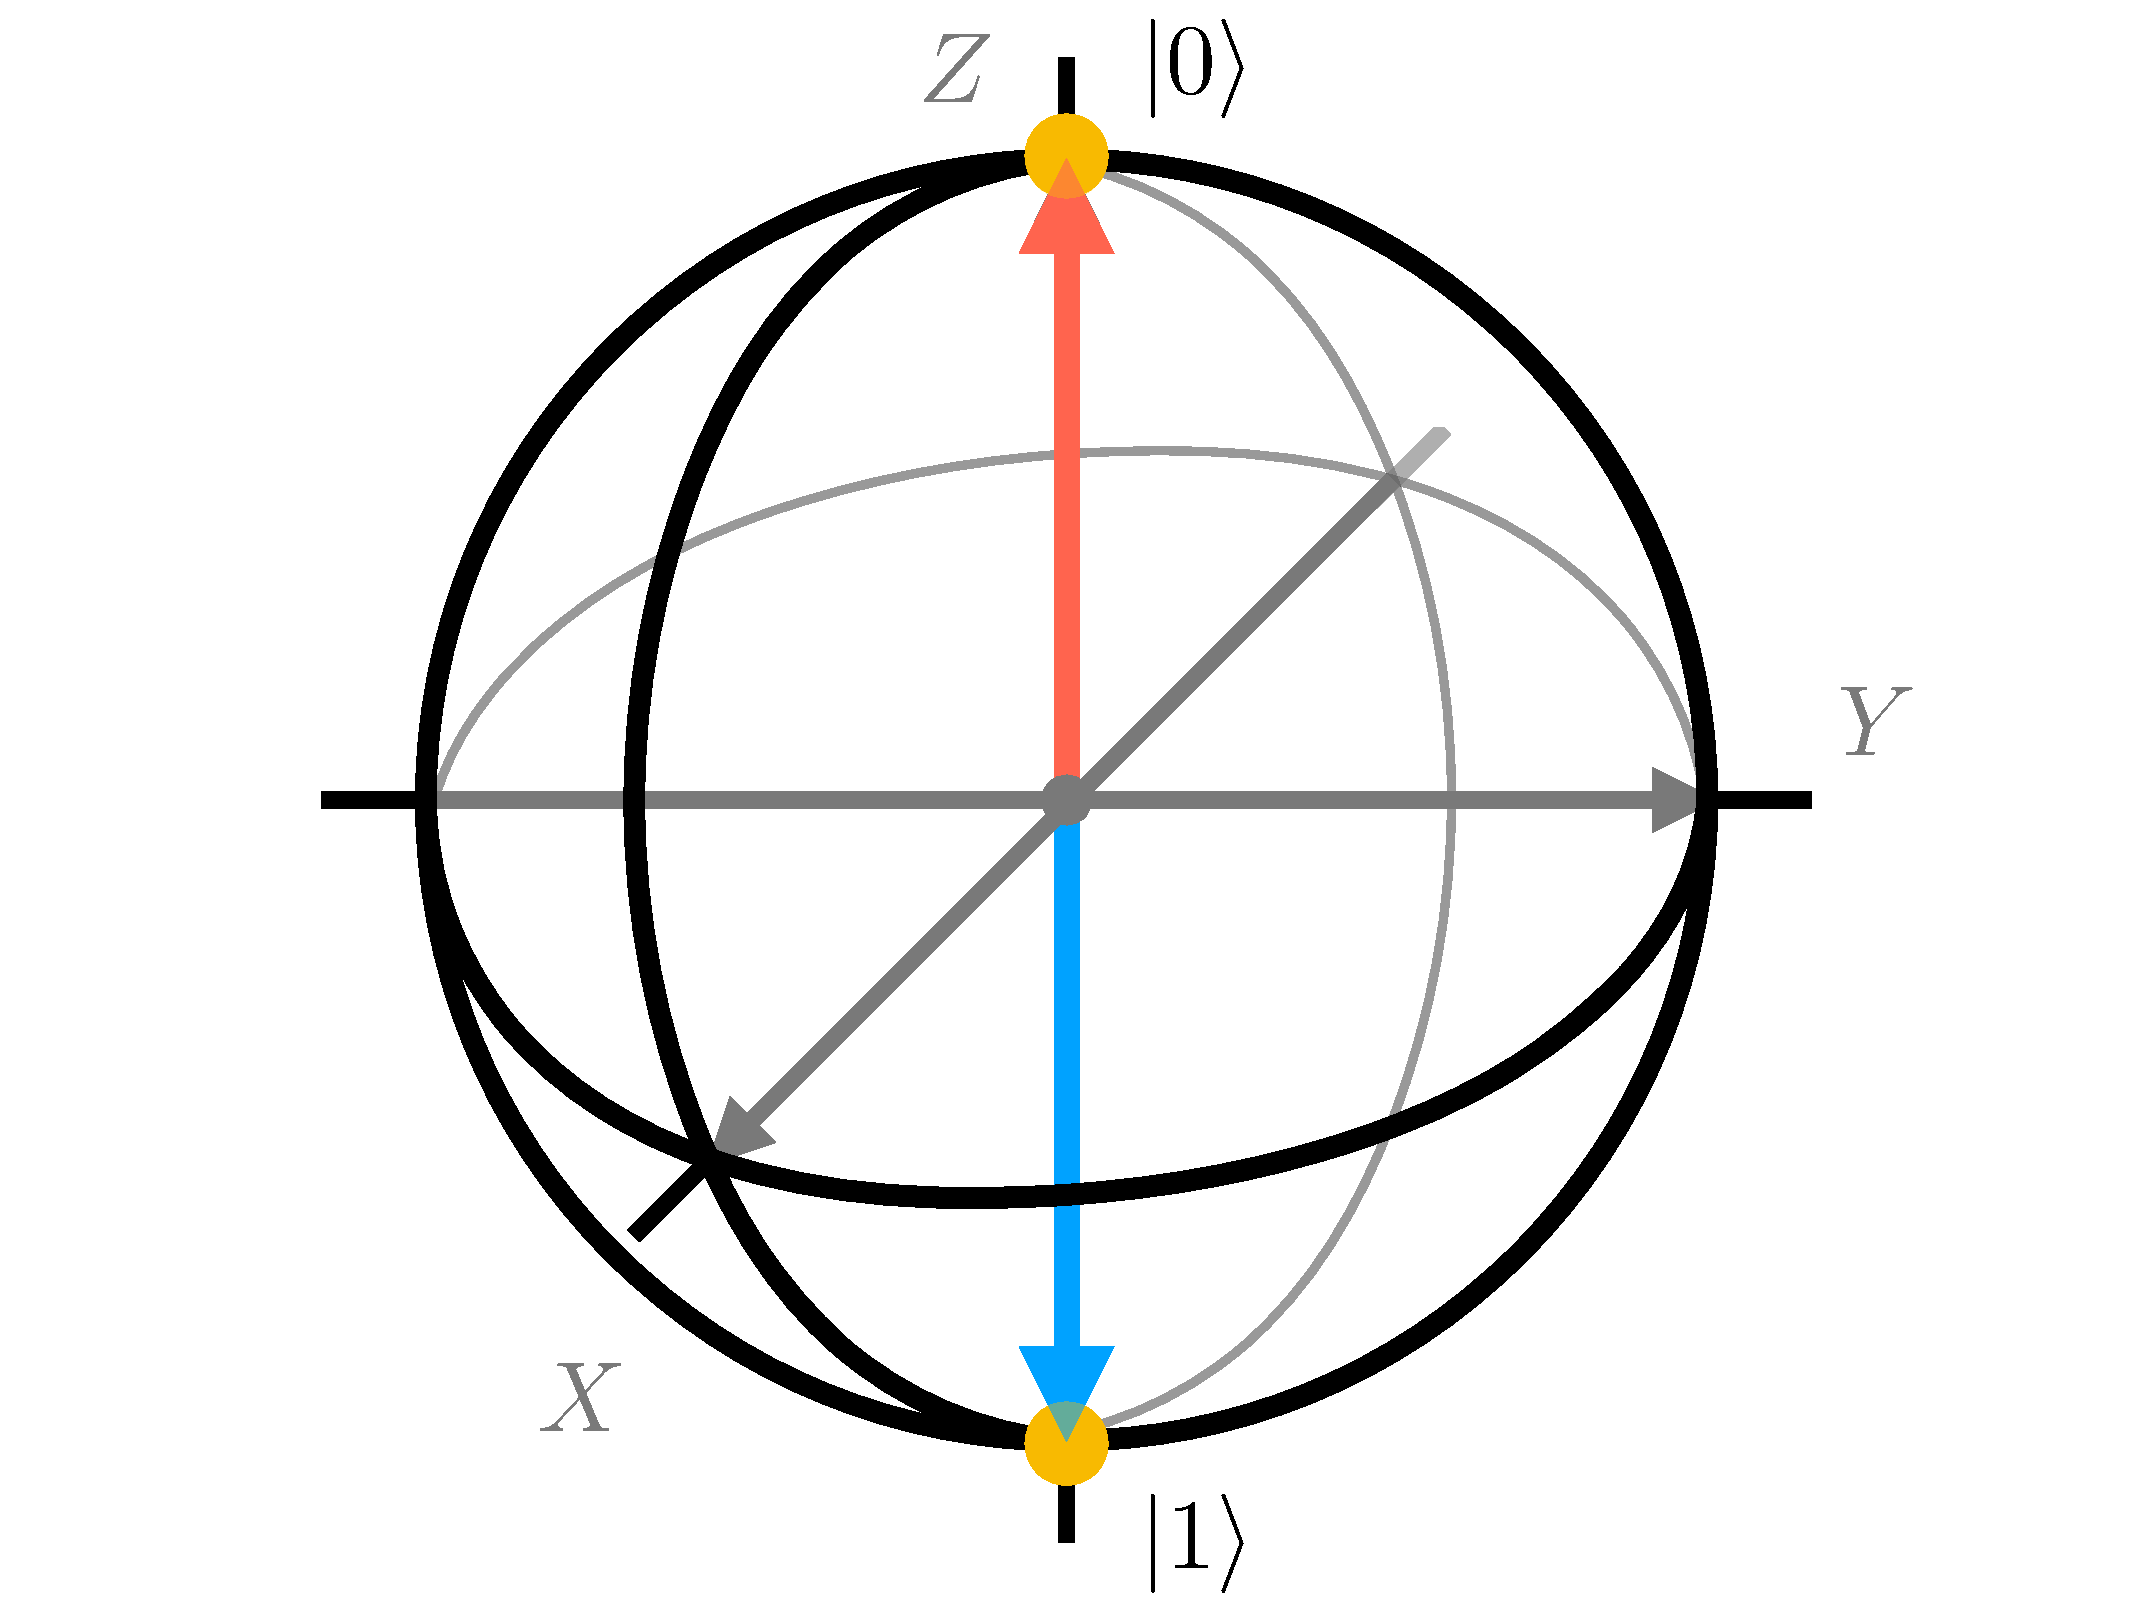
\includegraphics[width=.25\paperwidth]{Figures/chapter01/bloch-sphere}
    \end{center}

  \end{multicols}

  % which means that it acts with zero eigenvalue on even parity states, and as Pauli~Y in the subspace $\qty{\ket{\bin 10}, \ket{\bin 01}}$. As we will see, this implies that the evolution associated to the kinetic term can only create or annihilate particle-antiparticle pairs on a single physical site (i.e. $H_N^{(1)}$), or between nearest neighbors (i.e. $H_N^{(3)}$); enabling motion along the lattice, and hinting at a necessary number of rotations being proportional to the number of physical lattice sites (i.e. to allow pairs to completely cycle around the lattice), which in turn implies an efficient polynomial parametrization of Hilbert space. Moreover, it also ensures that single-particle states are unreachable and therefore charge is conserved, which is consistent with all that we know about QCD. The boundary term with the string will be similar but rotating on $\qty(\bigotimes Z) Y$ instead of just on $Y$.

%% ----------------------------------------------------------------------------
\break
%% ----------------------------------------------------------------------------

  \begin{minipage}[c]{\linewidth}
  \vspace{-1em}
  \footnotesize{\begin{align*}
    H_{N}^{(1)} \;\defeq\;&
      \frac{1}{4a} \sum_\alpha \sum_{n=\text{even}}^{2N-1}
      \qty[
        \sigma_\alpha^{1}(n+1) \sigma_\alpha^{2}(n) -
        \sigma_\alpha^{2}(n+1) \sigma_\alpha^{1}(n)
      ] \qc\\
    H_{N}^{(3)} \;\defeq\;&
      \frac{1}{4a} \sum_\alpha \sum_{n=\text{odd}}^{2N-2}
      \qty[
        \sigma_\alpha^{1}(n+1) \sigma_\alpha^{2}(n) -
        \sigma_\alpha^{2}(n+1) \sigma_\alpha^{1}(n)
      ] +\\&
      \frac{1}{4a} \sum_\alpha \!
      \qty[\prod_{l=1}^{2N-2} \!\! \sigma_\alpha^3(l)] \!
      \qty[
        \sigma_\alpha^{1}(0) \sigma_\alpha^{2}(2N \!-\! 1) -
        \sigma_\alpha^{2}(0) \sigma_\alpha^{1}(2N \!-\! 1)
      ]
  \end{align*}}
  \vspace{-1em}
  \begin{figure}[!p]
  	\centering
  	\begin{minipage}[c]{.20\linewidth}
  		\centering
  		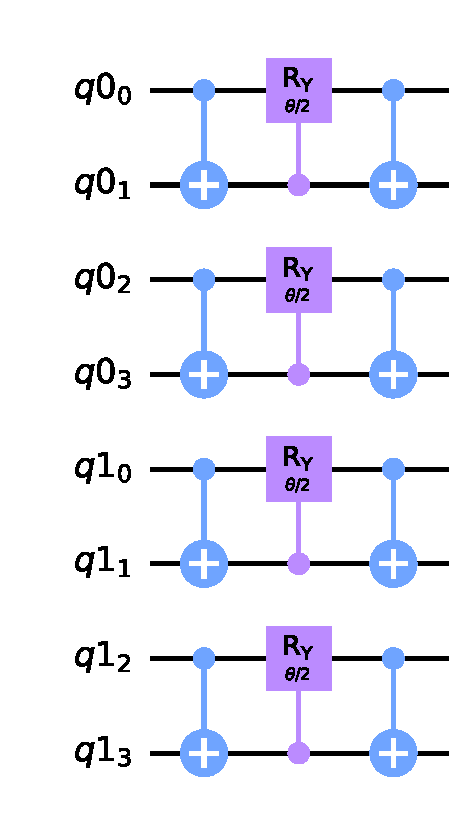
\includegraphics[height=15em]{Figures/chapter06/H1-rotation}
  	\end{minipage}
  	\hspace{1em}
  	\begin{minipage}[c]{.50\linewidth}
  		\centering
  		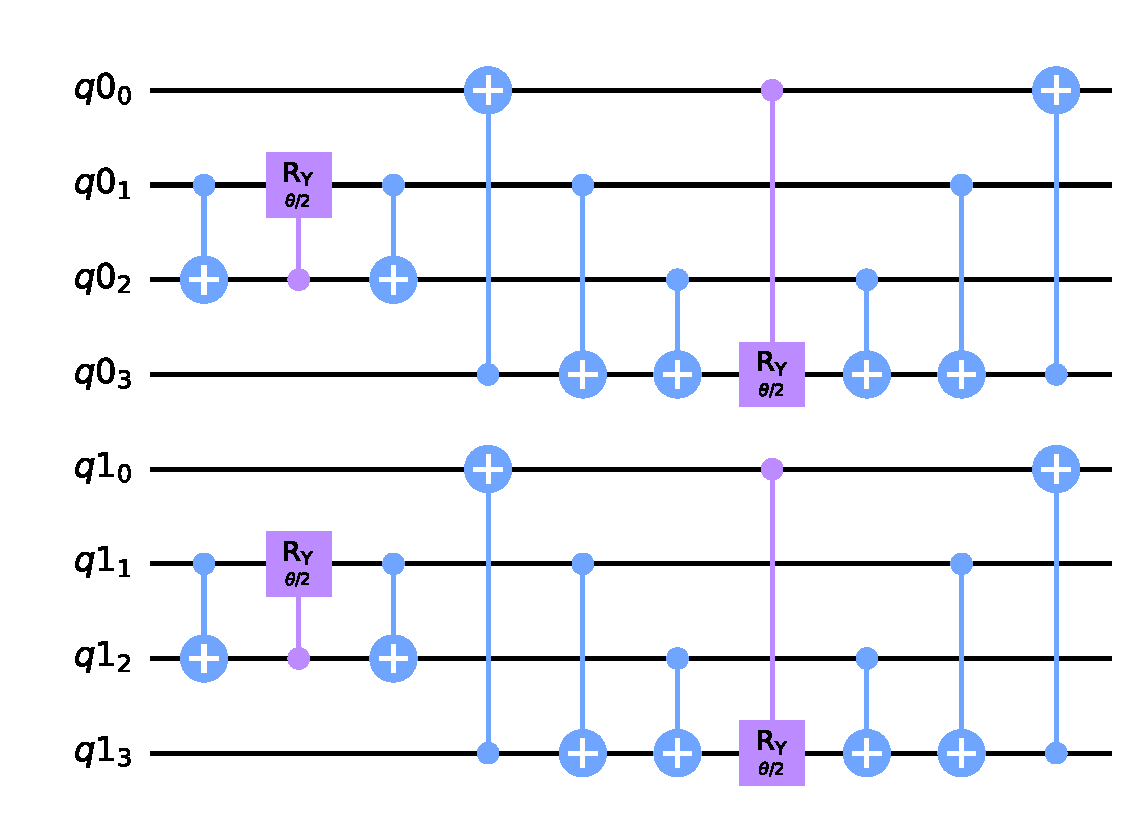
\includegraphics[height=15em]{Figures/chapter06/H3-rotation}
  	\end{minipage}
  \end{figure}
  \vspace{-2em}
  \end{minipage}


\end{frame}

%% ----------------------------------------------------------------------------
%% ----------------------------------------------------------------------------

\subsection{Ground/hadron states}

%% ----------------------------------------------------------------------------
%% ----------------------------------------------------------------------------

\begin{frame}{Ground and hadron states ($N=3$, $N_\text{flavor}=2$)}

  \begin{figure}[!p]
  	\centering
  	\begin{minipage}[c]{.40\linewidth}
  		\centering
  		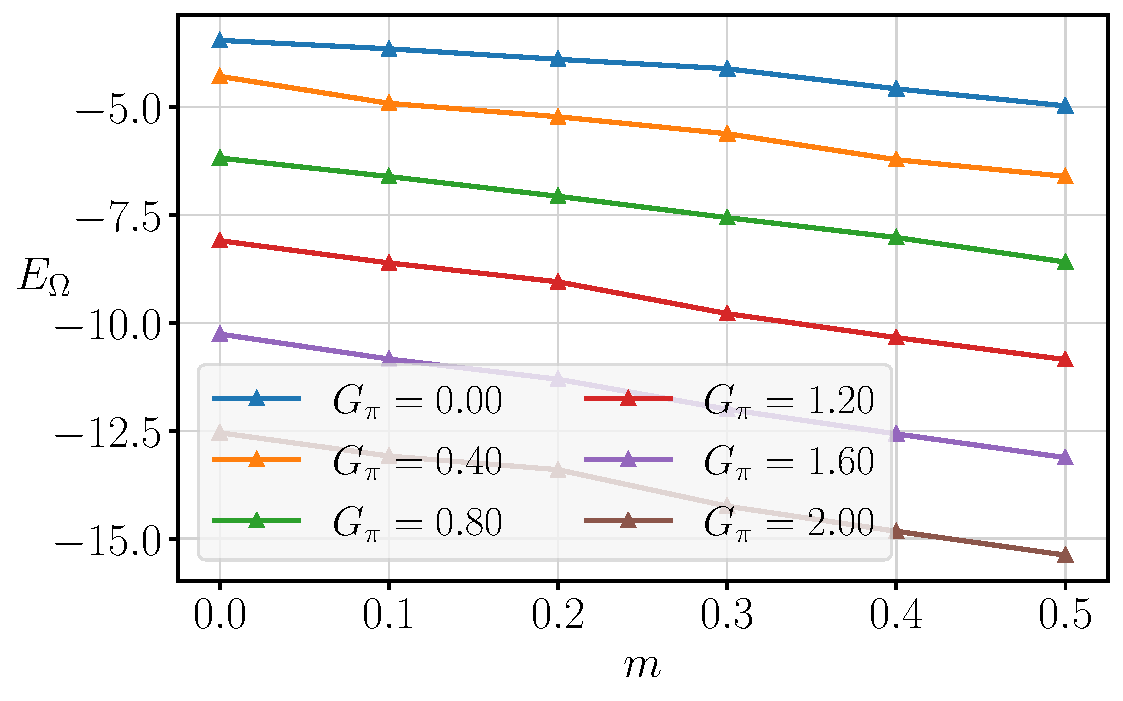
\includegraphics[width=\linewidth]{Figures/chapter06/g-Ev-curves}
  	\end{minipage}
    \hspace{.025\linewidth}
  	\begin{minipage}[c]{.40\linewidth}
  		\centering
  		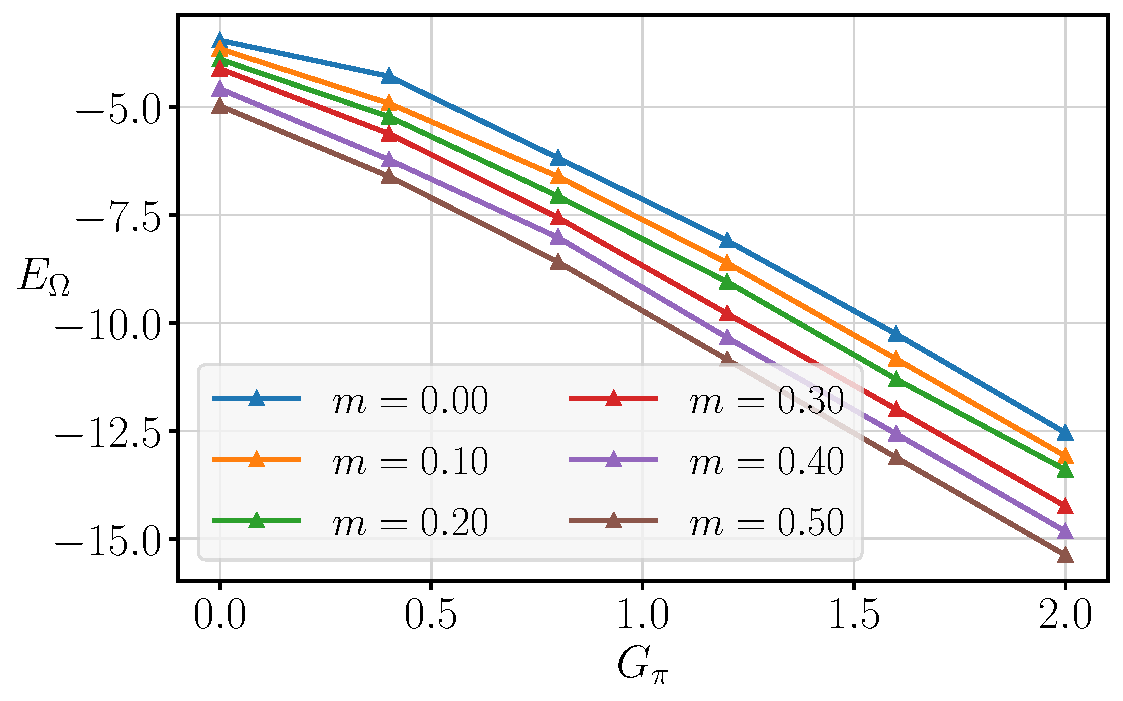
\includegraphics[width=\linewidth]{Figures/chapter06/m-Ev-curves}
  	\end{minipage}
  \end{figure}

  \begin{figure}[!p]
  	\centering
  	\begin{minipage}[c]{.40\linewidth}
  		\centering
  		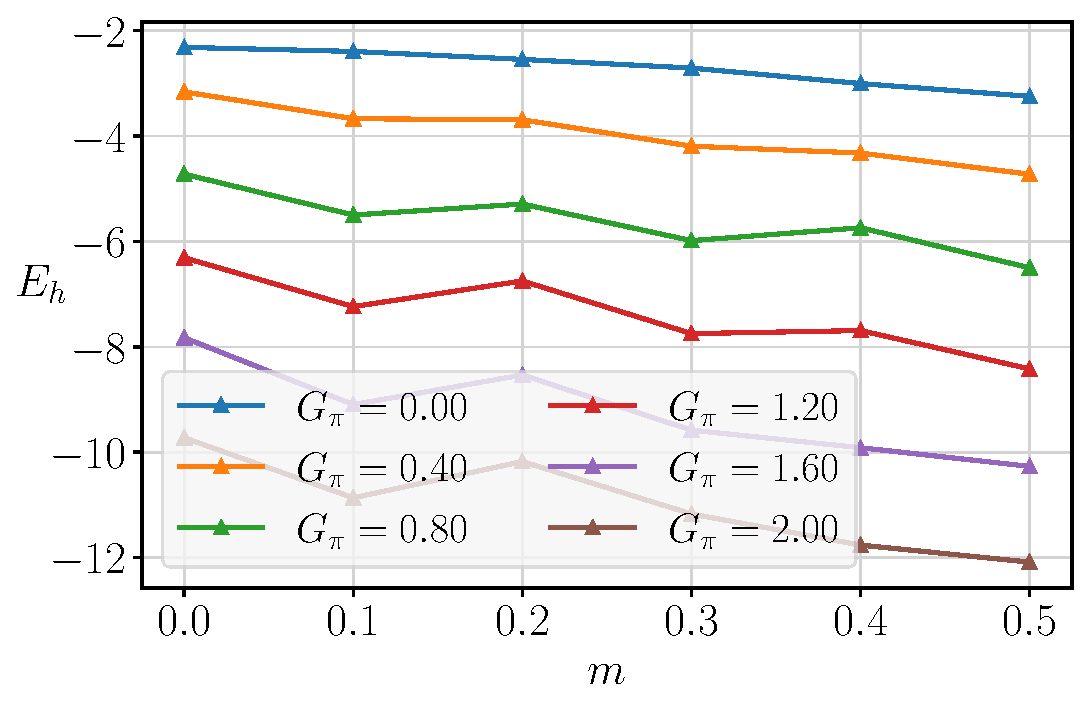
\includegraphics[width=\linewidth]{Figures/chapter06/g-Eh-curves}
  	\end{minipage}
    \hspace{.025\linewidth}
  	\begin{minipage}[c]{.40\linewidth}
  		\centering
  		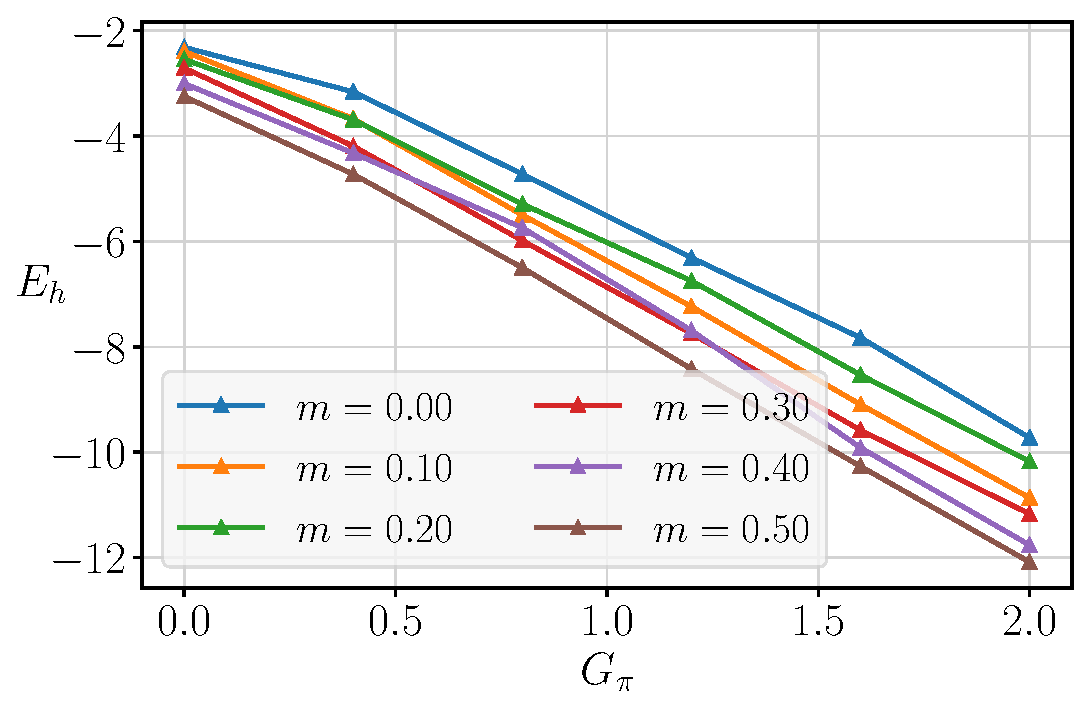
\includegraphics[width=\linewidth]{Figures/chapter06/m-Eh-curves}
  	\end{minipage}
  \end{figure}

\end{frame}
%% ----------------------------------------------------------------------------
%% ----------------------------------------------------------------------------

\subsection{Mass generation}

%% ----------------------------------------------------------------------------
%% ----------------------------------------------------------------------------

\begin{frame}[allowframebreaks]{Mass generation ($N=3$, $N_\text{flavor}=2$)}

  With these results, we can now obtain the hadron's mass as the difference between the hadron's energy and the computed vacuum energy:

  \begin{gather*}
    M \defeq \mel{h}{H_N}{h} - \mel{\Omega}{H_N}{\Omega} \qd
  \end{gather*}

  \begin{figure}[!p]
  	\centering
  	\begin{minipage}[c]{.40\linewidth}
  		\centering
  		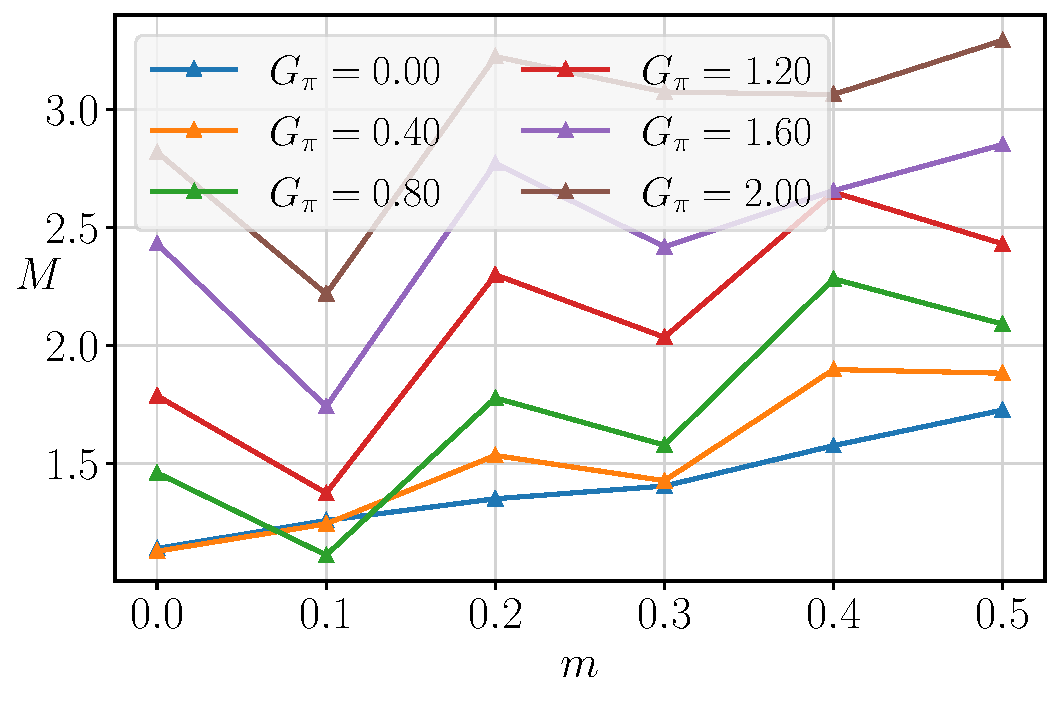
\includegraphics[width=\linewidth]{Figures/chapter06/g-mass-curves}
  	\end{minipage}
    \hspace{.025\linewidth}
  	\begin{minipage}[c]{.40\linewidth}
  		\centering
  		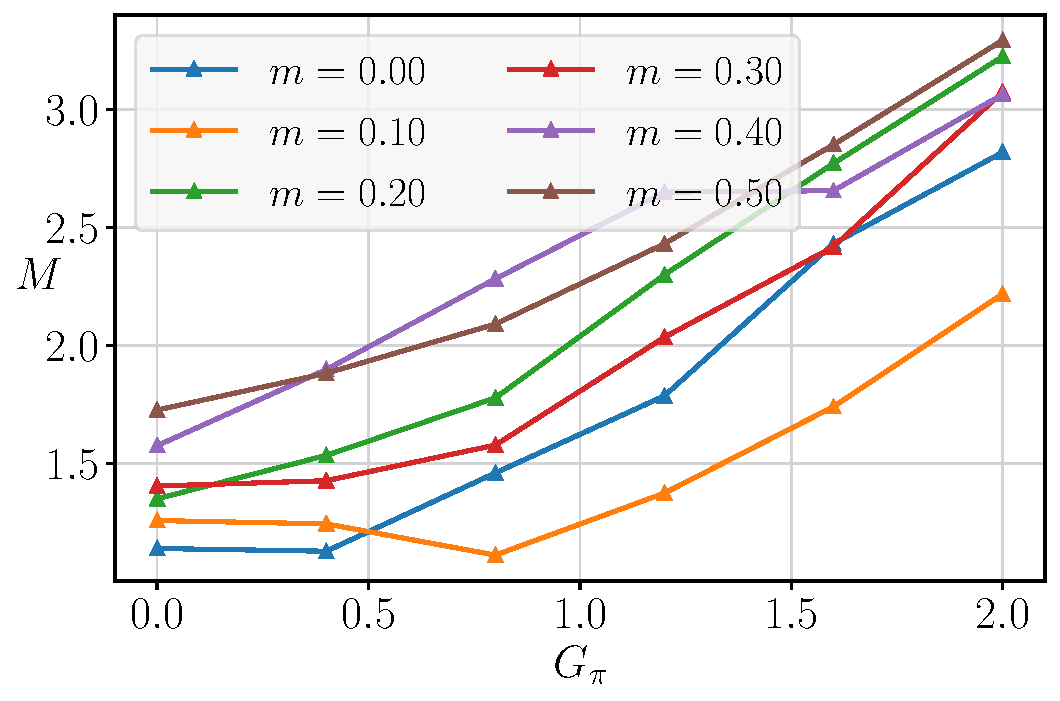
\includegraphics[width=\linewidth]{Figures/chapter06/m-mass-curves}
  	\end{minipage}
  \end{figure}

%% ----------------------------------------------------------------------------
\break
%% ----------------------------------------------------------------------------

  Nonetheless, we can see this more clearly by introducing a new metric. To motivate its definition, let us first define the different contributions to the mass of the hadron as:

  \begin{align*}
    M   \;\defeq\;&
      M_M + M_K + M_G \qc\\
    M_M \;\defeq\;&
      \mel{h}{H_N^{(M)}}{h} - \mel{\Omega}{H_N^{(M)}}{\Omega} \qc\\
    M_K \;\defeq\;&
      \mel{h}{H_N^{(K)}}{h} - \mel{\Omega}{H_N^{(K)}}{\Omega} \qc\\
    M_G \;\defeq\;&
      \mel{h}{H_N^{(G)}}{h} - \mel{\Omega}{H_N^{(G)}}{\Omega} \qd
  \end{align*}

  Our goal here is to compare the component of mass associated with interactions $M_G$, and that associated with the quark masses $M_M$. It is then natural to define:

  \begin{gather*}
    \mathcal{M}(m,G_\pi) \;\defeq\; \frac{M_G - M_M}{M} \qc
  \end{gather*}

%% ----------------------------------------------------------------------------
\break
%% ----------------------------------------------------------------------------

  From which we can distinguish three regimes:

  \begin{align*}
    M   \;\approx\;& M_G \qRa \mathcal{M} \approx +1 \qc\\
    M   \;\approx\;& M_M \qRa \mathcal{M} \approx -1 \qc\\
    M_G \;\approx\;& M_M \qRa \mathcal{M} \approx  0 \qd
  \end{align*}

  \begin{figure}[!tbp]
  	\centering
  	\begin{minipage}[c]{.40\linewidth}
  		\centering
  		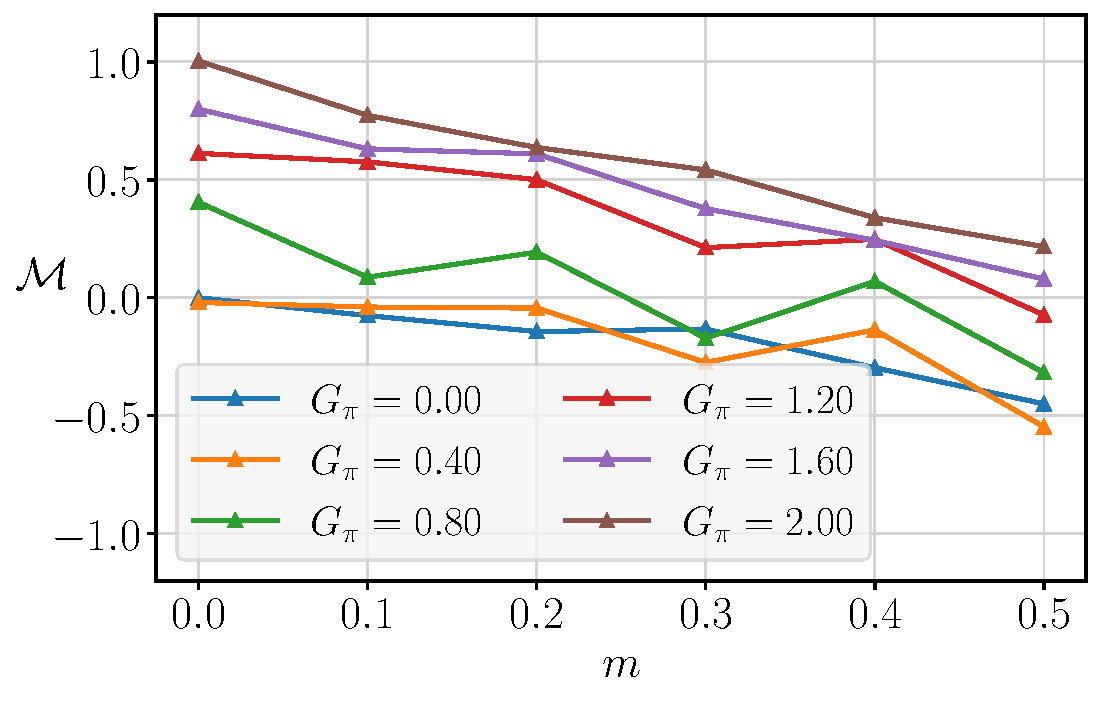
\includegraphics[width=\linewidth]{Figures/chapter06/g-ratio-curves}
  	\end{minipage}
    \hspace{.025\linewidth}
  	\begin{minipage}[c]{.40\linewidth}
  		\centering
  		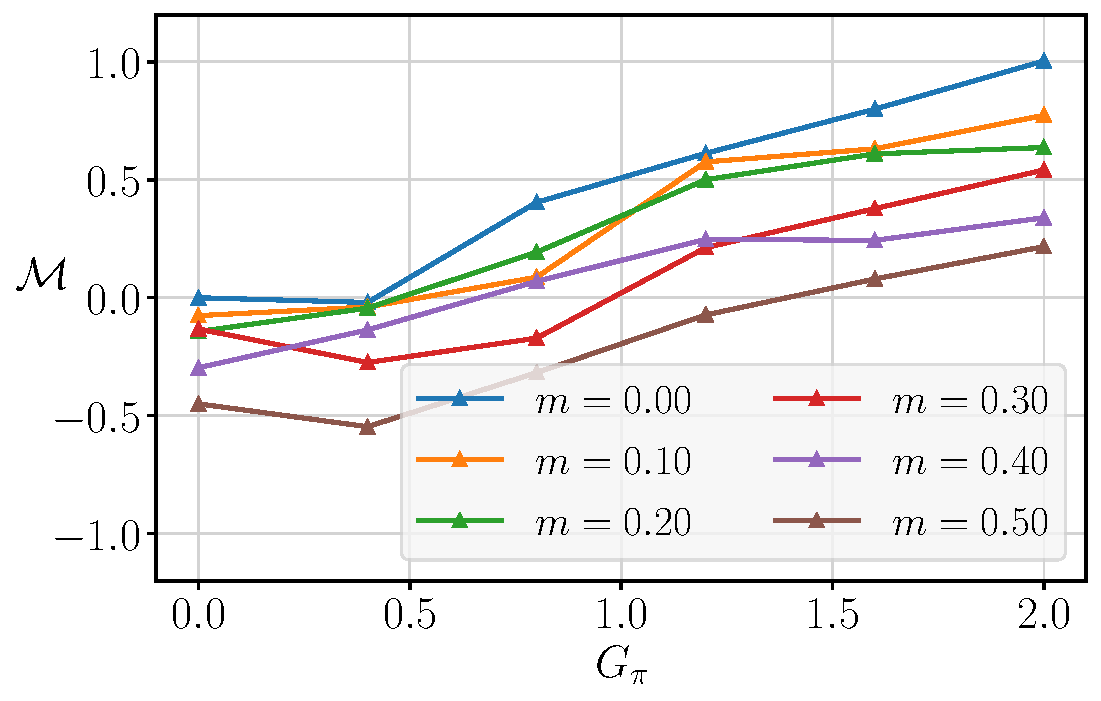
\includegraphics[width=\linewidth]{Figures/chapter06/m-ratio-curves}
  	\end{minipage}
  \end{figure}

\end{frame}
